\documentclass[onecolumn, draftclsnofoot,10pt, compsoc]{IEEEtran}
\usepackage{graphicx}
\usepackage{url}
\usepackage{setspace}
\usepackage{float}
\usepackage{geometry}
\usepackage{etoolbox}
\usepackage{enumitem}% http://ctan.org/pkg/enumitem
\makeatletter

\geometry{textheight=9.5in, textwidth=7in}

% 1. Fill in these details
\def \CapstoneTeamName{		Team 45}
\def \CapstoneTeamNumber{		45}
\def \GroupMemberOne{			McIntyre Santa Cruz}
\def \GroupMemberTwo{			Blake Hudson}
\def \GroupMemberThree{			Sean Cramsey}
\def \CapstoneProjectName{		Autodesk Predictive Analytics}
\def \CapstoneSponsorCompany{	Autodesk, Inc}
\def \CapstoneSponsorPerson{		Andrew Faix}

% 2. Uncomment the appropriate line below so that the document type works
\def \DocType{	
				Requirements Document
				%Technology Review
				%Design Document
				%Progress Report
				}
			
\newcommand{\NameSigPair}[1]{\par
\makebox[2.75in][r]{#1} \hfil 	\makebox[3.25in]{\makebox[2.25in]{\hrulefill} \hfill		\makebox[.75in]{\hrulefill}}
\par\vspace{-12pt} \textit{\tiny\noindent
\makebox[2.75in]{} \hfil		\makebox[3.25in]{\makebox[2.25in][r]{Signature} \hfill	\makebox[.75in][r]{Date}}}}
% 3. If the document is not to be signed, uncomment the RENEWcommand below
\renewcommand{\NameSigPair}[1]{#1}

%%%%%%%%%%%%%%%%%%%%%%%%%%%%%%%%%%%%%%%
\begin{document}
\begin{titlepage}
    \pagenumbering{gobble}
    \begin{singlespace}
    	\includegraphics[height=4cm]{coe_v_spot1}
        \hfill 
        % 4. If you have a logo, use this includegraphics command to put it on the coversheet.
        %\includegraphics[height=4cm]{CompanyLogo}   
        \par\vspace{.2in}
        \centering
        \scshape{
            \huge CS Capstone \DocType \par
            {\large\today}\par
            \vspace{.5in}
            \textbf{\Huge\CapstoneProjectName}\par
            \vfill
            {\large Prepared for}\par
            \Huge \CapstoneSponsorCompany\par
            \vspace{5pt}
            {\Large\NameSigPair{\CapstoneSponsorPerson}\par}
            {\large Prepared by }\par
            Group\CapstoneTeamNumber\par
            % 5. comment out the line below this one if you do not wish to name your team
            \CapstoneTeamName\par 
            \vspace{5pt}
            {\Large
                \NameSigPair{\GroupMemberOne}\par
                \NameSigPair{\GroupMemberTwo}\par
                \NameSigPair{\GroupMemberThree}\par
            }
            \vspace{20pt}
        }
        \begin{abstract}
        % 6. Fill in your abstract    
        	Autodesk Inventor is commercial software that lends itself to numerous industries. This is due to its ability to digitally model actual products that will eventually be put into production. To accurately reflect what a user of Inventor has created, there exist  many options when it comes to command inputs that will hopefully result in a desired outcome. Due to wide array of uses, the user base is incredibly diverse and each user generally has a unique set of tasks that they perform frequently. Although this may be the case, the user interface is standard for all users. This means that a command’s location on the screen and hotkeys are the same for every user no matter how frequently they are employed. Autodesk has therefore set out to make using Inventor easier for its existing user base by developing a software add-in that will learn from a specific users inputs and predict what command the user is most likely to use next. This prediction will be presented to the user and will eventually assist in reducing time spent completing a task.  (\url{https://tobi.oetiker.ch/lshort/lshort.pdf})
        \end{abstract}     
    \end{singlespace}
\end{titlepage}
\newpage
\pagenumbering{arabic}
\tableofcontents
% 7. uncomment this (if applicable). Consider adding a page break.
%\listoffigures
%\listoftables
\clearpage

% 8. now you write!
\section{Introduction}

Chapter one delivers what the document contains. Along with definitions and abbreviations for the language used in the document. The topics that will be discussed is the scope of the software developed  

\subsection{Purpose}

The purpose of this document is to define the requirements needed for the development of an Autodesk Inventor Command add-in. Once defined, the requirements will be explored and properly outlined. 

\subsection{Scope}

The Autodesk Inventor Command add-in is an addition to the already existing framework of the Inventor application. The add-in being discussed will gather inputs from a user and will make a visual suggestion of the next command a user will most likely enter. The add-in will be limited to functioning within the sketch mode found within Inventor. Upon completion of the application, users will complete tasks with fewer inputs required, and in less time. 

\subsection{Glossary}
\begin{itemize}
    \item Add-in - A special type of Inventor program. Add-ins are automatically started whenever Inventor is run. This results in add-ins having the capability to insert itself into Inventor’s user interface, and to interact and respond to events within Inventor
    \item AICA - Acronym for Autodesk Inventor Command add-in
    \item Assembly - In Inventor, assembly is a collection of parts [3]. 
    \item Autodesk - An American multinational software corporation that develops software for the architecture, engineering, construction, manufacturing, media, and entertainment industries.
    \item Autodesk Inventor - Software developed by Autodesk. It is a computer-aided design(CAD) application for 3D mechanical design, simulation, visualization, and documentation.
    \item Drawing - In Inventor, drawing is referred to as a blueprint of the assembly [3].
    \item Machine Learning - A method to analyze data that results in a predictive model. This is a form of artificial intelligence that can learn to identify patterns based on available data and to ultimately make decisions based on its own analysis.
    \item Part - In Inventor, a part is a small 3D or 2D component [3].
    \item Presentation - In Inventor, a presentation expands an assembly to view each individual part. It is used to see the product with each individual part [3].
    \item RNN - Acronym for recurrent neural network. It is a class of artificial neural networks. The type of neural network utilizes temporal dynamic behavior for a time sequence. This allows internal states to process sequences of inputs [2].
    \item Sketch Mode - Feature found within Autodesk Inventor. Allows a user to digitally sketch their product.
    \item XML - Extensible Markup Language. Primarily used to store and transport data. It is essentially a formatting style that has been standardized and can therefore be deconstructed quickly by the appropriate software.

\end{itemize}


\subsection{References}
[1] “3D CAD Software for Product Development.” Inventor | Mechanical Design & 3D CAD Software | Autodesk, www.autodesk.com/products/inventor/overview.\newline
\newline
[2]{ “Recurrent Neural Network.” Wikipedia, Wikimedia Foundation, 25 Oct. 2018, en.wikipedia.org/wiki/Recurrent_neural_}\newline
networknetwork.\newline\newline
[3]${ “File Types and Templates in Inventor.” Autodesk Support & Learning, knowledge.autodesk.com/support/inventor-products/getting-started/caas/CloudHelp/cloudhelp/2014/ENU/Inventor/files/GUID-94B779C0-6B2B-499A-A4F9\newline
-2E4BAB49712F-htm.html.}$

\section{Overall Description}
The purpose of this section is to define how the Autodesk Inventor Command add-in relates to the overall system of Autodesk Inventor. It will also be a piece used to fully explain how the software functions and makes use of foreign libraries in order to accomplish its predictive goal. Finally the software will be placed in context, and possible User interactions will be fully explored.   

\subsection{Product Perspective}
The form this software has taken is that of an Autodesk Inventor add-in. This add-in is run from within Inventor, and essentially becomes an extension of the existing system. The nature of an add-in being run from within Inventor means that any event which occurs from within Inventor can be responded to by an add-in. In the case of the AICA, all commands entered during the use of sketches in Inventor will be recorded into an XML database. The add-in itself will contain a machine learning algorithm that will learn from these stored user inputs. A visual suggestion will appear within Inventor, in the form of a pop-up, regarding the users next command needed that has been generated by a machine learning algorithm.

    \begin{figure}[H]
        \centering
         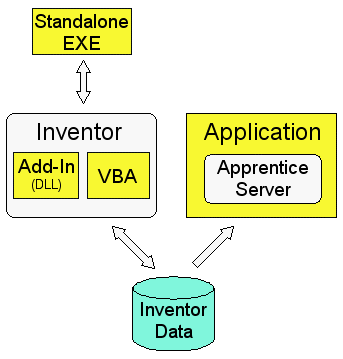
\includegraphics{APIMethods.png}
        \caption{Inventor API}
        \label{fig:1}
    \end{figure}
   


\subsection{Product Functions}
The product will provide users with suggested commands which are generated based upon the users previous usage.  This system will develop its functionality without direct interactions with the user.  Over time this product should develop to be tailored to the users practices, allowing for the user to enhance their productivity by minimizing the time spent on repeated tasks. The suggested command itself will make an appearance within the user interface.

\subsection{User Characteristics}
In general, the user base of Autodesk Inventor consists of customers who have used the software for years and are familiar with how to complete the tasks they have set for themselves. This means that the target user for this product is someone who is well versed in what commands are available to them and exactly what each command does. Inventor as a software has numerous different uses which results in a wide variety of users, along with the reason for choosing Inventor. The one constant will be their high level of skill in what they commonly use Inventor for. 

\subsection{Limitations}The Autodesk Inventor application is a large piece of software, requiring a significant portion of power to run. With the inclusion of a program that will constantly be taking inputs and processing them in order to make a suggestion, which could lead to processes taking a noticeably long time. This would defeat the purpose of the add-in if the suggestion takes to long to be presented to the user. Another limitation is the library used to develop the machine learning algorithm must work alongside the Autodesk Inventor API. 

\subsection{Assumptions and Dependencies}
Our assumption is that a user will use the sketch mode for a significant amount of time, and make use of a significant amount of commands in order to justify the development of this add-in. 

A dependency will be the requirement that a user has the Autodesk Inventor software installed. 

\subsection{Apportioning of Requirements}
The following graphic outlines our proposed agenda for the projects duration.  While it is expected that all tasks will be completed within their allotted times, overflow periods have been included into this timeline.
\newline
    \begin{figure}[H]
        \centering
         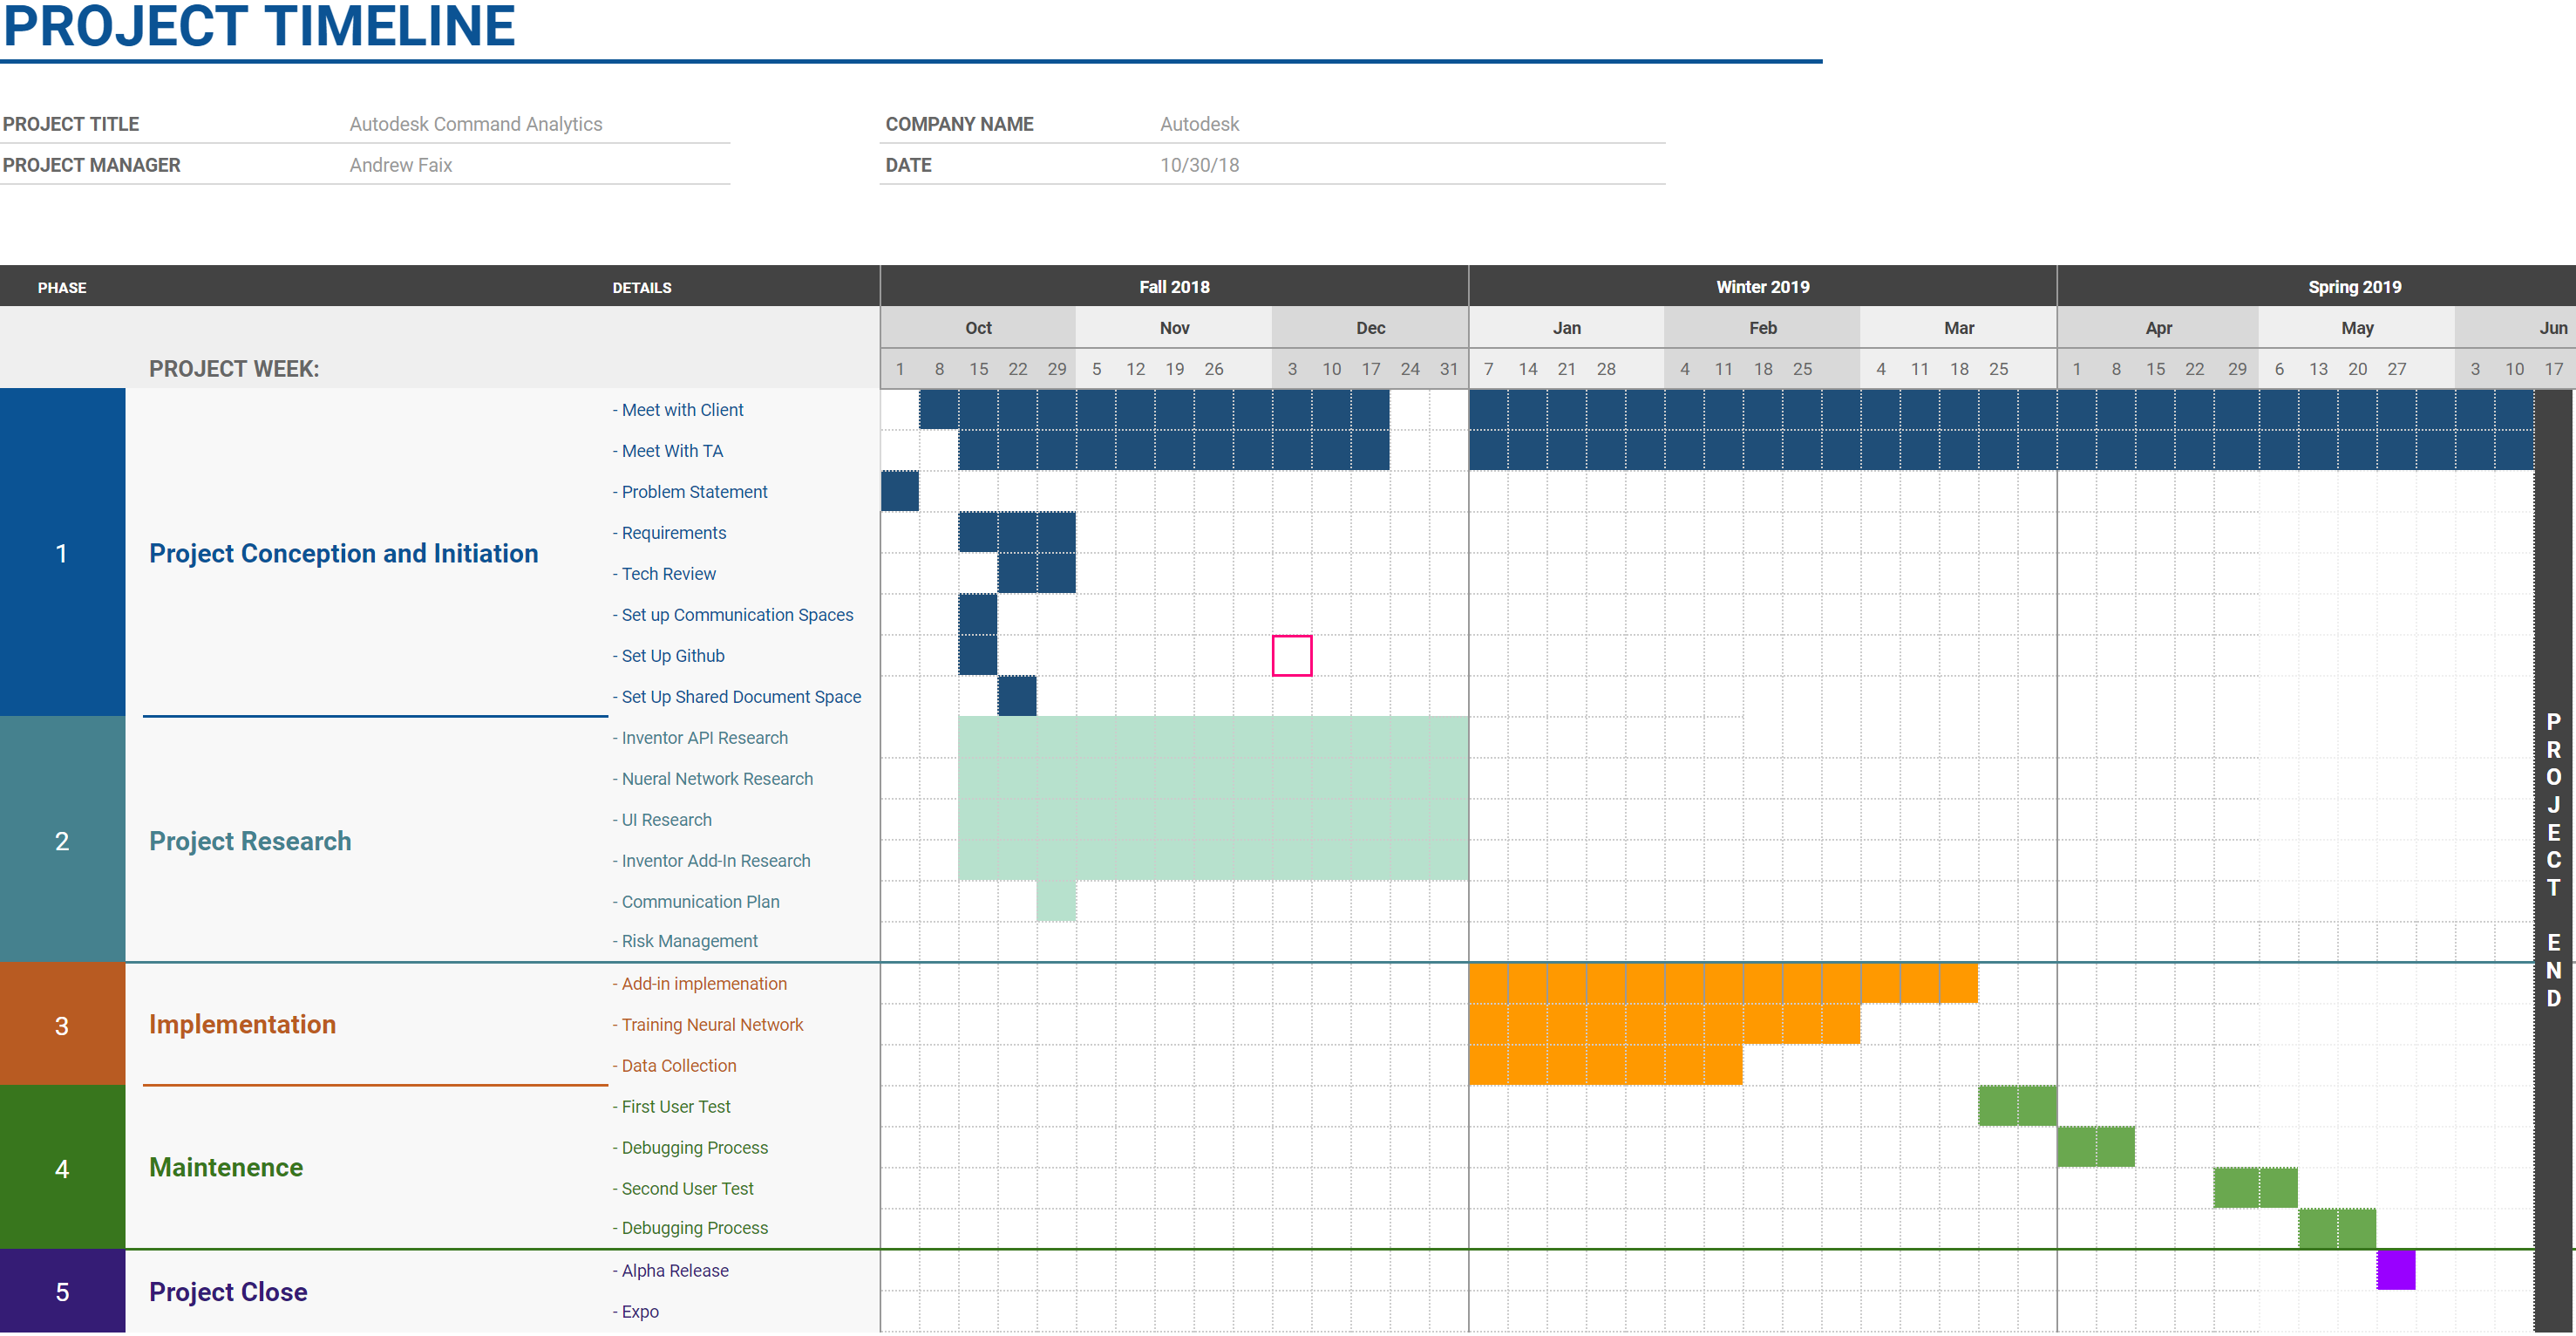
\includegraphics[scale=0.22]{GANTT_0.png}
        \caption{GANTT Chart}
        \label{fig:2}
    \end{figure}

\section{Specific Requirements}
This section will contain a description of all functional and nonfunctional requirements for the Autodesk Inventor Command add-in. Details on the features of the add-in in question will be fully examined.

\subsection{Functional Requirements}
This section defines functional requirements applicable to the systems requirements.
\newline
\newline
\textbf{ID: FR1}
\newline
TITLE: Download Autodesk Inventor
\newline
DESC: The application is accessible from the Autodesk website [1]. 
\newline
RAT:  The user must have access to the base software package in order for the add-in to be of any benefit.
\newline
DEPEND: None
\newline
\newline
\textbf{ID: FR2}
\newline
TITLE: Download add-in 
\newline
DESC: Download the add-in from the Autodesk store.
\newline
RAT:  The add-in must be available and be able to easily link with the Inventor application.
\newline
DEPEND: FR1
\newline
\newline
\textbf{ID: FR3}
\newline
TITLE: Open the Autodesk Inventor executable 
\newline
DESC: A user should start the application. Depending on new users, a tutorial will appear.\newline
RAT: This is where interaction with the Inventor environment occurs.  \newline
DEPEND: FR1\newline
\newline
\textbf{ID: FR4}\newline
TITLE: Create new design\newline
DESC: A user should click the new button in the top left corner of the interface\newline
RAT: Allows the user to create a new project.\newline
DEPEND: FR1, FR2\newline
\newline
\textbf{ID: FR5}\newline
TITLE: Project Management Menu \newline
DESC: A project management menu will give a selection to create a part, assembly, drawing, or presentation in 2D or 3D. \newline
RAT: In order for the user to select what type of project they are working on.\newline
DEPEND: FR3\newline
\newline
\textbf{ID: FR6}\newline
TITLE: Utilize commands\newline
DESC: The user will begin designing their object using Inventor commands\newline
RAT: In order for the user to create designs and use the downloaded add-in\newline
DEPEND: FR5\newline
\newline
\textbf{ID: FR7}\newline
TITLE: Predictive Analytics\newline
DESC: Our add-in will begin to generate predicted commands based on a sequence of the users commands. \newline
RAT: The add-in will need input in order to generate predicted commands.\newline
DEPEND: FR6, FR2\newline
\newline
\textbf{ID: FR8}\newline
TITLE: Stretch Goal for FR7\newline
DESC: A command will pop up in near the cursor with the predicted command.\newline
RAT: This will aid the user to become more efficient with Inventor commands.\newline
DEPEND: FR7, FR6, FR2\newline
\newline

\subsection{Performance Requirements}
\textbf{ID: QR1}\newline
TITLE: Predictive Speed\newline
DESC: The system will take no longer then 3 seconds to visually display to the user the predicted command\newline
RAT: In order for the user to in fact increase productivity by lessening work time\newline
DEPEND: None\newline
\newline
\textbf{ID: QR2}\newline
TITLE: Visual Understanding\newline
DESC: The system will display the predicted command in an easy to understand method. \newline
RAT: In order for the user to clearly understand what the system is recommending\newline
DEPEND: None\newline
\newline
\textbf{ID: QR3}\newline
TITLE: Data Testability\newline
DESC: The system will be easy to grade on accuracy due to the nature of a user choosing to follow the systems recommendation or to choose another option.\newline
RAT: The system will know when it has predicted correctly or not\newline
DEPEND: None\newline
\newline
\textbf{ID: QR4}\newline
TITLE: Runtime Minimization\newline
DESC: The effect upon the main applications normal runtime must be minimal.\newline
RAT: If the main application is slowed by the addition of this add-in then its core purpose is rendered null.\newline
DEPEND: None\newline
\subsection{Design Constraints}
The add-in solution is a local tool. That is to say that all data available will be locally collected and stored. The algorithm used to make command prediction will therefore only be able to learn from one specific source. The underlying specification for the add-in is to work faster than the user selecting the command from the current UI toolbar. This will put time constraints on how fast the algorithm will retrieve a predicted command. Thus, the final algorithm should have an efficient calculated running time. 
\end{document}